\chapter{Navigation}
\label{ch:navigation}

\pkg{dharma_navigation} plans paths on the site map, loads taught routes, follows paths around
people and runs reactive avoidance. Its velocity output is \topic{control/nav_cmd_vel} (the
launch default; never the robot's \topic{cmd_vel}, review F14/B2): the control mux decides what
reaches the robot.

\begin{center}
\begin{tabularx}{\textwidth}{@{}p{0.27\textwidth}X@{}}
  \toprule
  Node & Role \\
  \midrule
  \code{planner_node} & \topic{planner/go_to}: plan on \topic{/map}, hand the path to the
    follower, replan around blockages \\
  \code{path_loader_node} & \topic{navigation/load_path}: read a route CSV inside
    \param{sites_dir}, resample and smooth it (stop points never move), publish it latched \\
  \code{path_follower_node} & join, follow, final approach, stop points, pause reasons, motion
    guard; publishes \topic{control/nav_cmd_vel} \\
  \code{obstacle_avoidance_node} & a reactive policy on \topic{perception/sector_scan}
    $\to$ \topic{navigation/avoidance} \\
  \bottomrule
\end{tabularx}
\end{center}

\section{One braking model}
\label{sec:braking}

Every speed limit in the stack uses the model of \code{dharma_utils.safety}: from speed $v$,
with reaction time $\tr$ and deceleration $a$, the robot needs
\begin{equation}
  D(v) = v\,\tr + \frac{v^2}{2a}, \qquad\text{and the fastest speed that stops within } d
  \text{ is}\qquad v^*(d) = a\Big(-\tr + \sqrt{\tr^2 + \tfrac{2d}{a}}\Big),
  \label{eq:m-braking}
\end{equation}
with $v^*(d) = 0$ for $d \le 0$; the yaw-rate version uses the yaw deceleration and an angle. In
0.1 the path shift used $v = \sqrt{2a\,d}$ without the reaction time while the protective field
used $D(v)$ (finding N3); at 1.0~m of room the former allowed 0.78~m/s where 0.66~m/s was
right. The speed profile, the path shift, the motion guard and the protective field now share
\eqref{eq:m-braking}.

\section{Planner}

\subsection{Costmap}

\topic{/map} becomes a costmap at \param{costmap.resolution}: occupied cells (and unknown ones
with \param{costmap.unknown_is_obstacle}) are max-pooled onto the planning grid and live
obstacles of the safety scan can be stamped in. With the distance $d$ of a cell to the nearest
obstacle and the radii from the footprint (finding N1),
\begin{equation}
  r_\ell = r_{\mathrm{in}} + m, \qquad r_{\mathrm{c}}' = r_{\mathrm{c}} + m, \qquad
  R = \max(R_{\mathrm{infl}}, r_{\mathrm{c}}'),
\end{equation}
a cell is lethal for every heading when $d \le r_\ell$; between $r_\ell$ and $r_{\mathrm{c}}'$ a
collision depends on the heading and is checked with the oriented footprint; up to $R$ the cost
decays,
\begin{equation}
  c(d) = \begin{cases} \infty & d \le r_\ell\\[2pt]
  1 + W\,\dfrac{e^{-k(d - r_\ell)} - e^{-k(R - r_\ell)}}{1 - e^{-k(R - r_\ell)}} &
    r_\ell < d < R \\[8pt]
  1 & d \ge R \end{cases}, \qquad W = 5,\ k = \text{\param{costmap.cost_scaling}}.
\end{equation}

\subsection{Search}

A*~\cite{hart1968astar}, 8-connected without corner cutting; the step cost is the step length
times the cost of the target cell and $f = g + w\,h$ with the octile heuristic
$h = \max(\Delta_r, \Delta_c) + (\sqrt2 - 1)\min(\Delta_r, \Delta_c)$. Since $c \ge 1$, $h$ is
admissible for $w = 1$ (optimal paths); for $w > 1$ a path costs at most $w$ times the optimum.
A robot inside the inflation walks out of it (\param{search.start_escape}); a goal inside an
obstacle moves to the nearest cell within \param{search.goal_tolerance} where the robot fits at
the goal heading, and arrival is tested against that snapped goal (review F8).

\subsection{Post-processing and the footprint check}

Line-of-sight shortcuts are accepted only when the largest cost along the line does not exceed
that of the segment they replace; a line touching a cell corner counts both side cells, so it
never slips through a diagonal pinch (review F17). Waypoints are placed every
\param{search.spacing} and smoothed by gradient steps
$y_i \mathrel{+}= \alpha(x_i - y_i) + \beta(y_{i-1} + y_{i+1} - 2y_i)$, discarded when they touch
a lethal cell. Along the result, the oriented footprint is checked at the heading the follower
will use (the path direction, the goal heading at the end); where it does not fit, the cell is
blocked and the search runs again, up to \param{search.footprint_retries} times. For
non-holonomic robots a lattice or hybrid A* planner can be added behind the same interface.

\subsection{Goal session}

\topic{planner/go_to} plans, calls \topic{navigation/set_path} and \topic{navigation/start}, and
monitors the follower: \code{BLOCKED} for \param{monitor.replan_after_sec} or \code{OFF_PATH}
plans again with the obstacles of the safety scan, up to \param{monitor.max_replans}. A blind or
stale safety scan is never read as clear (review F1): the goal fails. Every failure after
\code{set_path} stops the follower (review F9). \topic{planner/cancel} has its own callback group
and a cancel flag checked between planning, \code{set_path} and \code{start} (review F10). The
pose is used only when TF is younger than \param{tf_timeout_sec}; a parameter change rebuilds
the costmap (review F15).

\section{Path follower}

\begin{figure}[h]
  \centering
  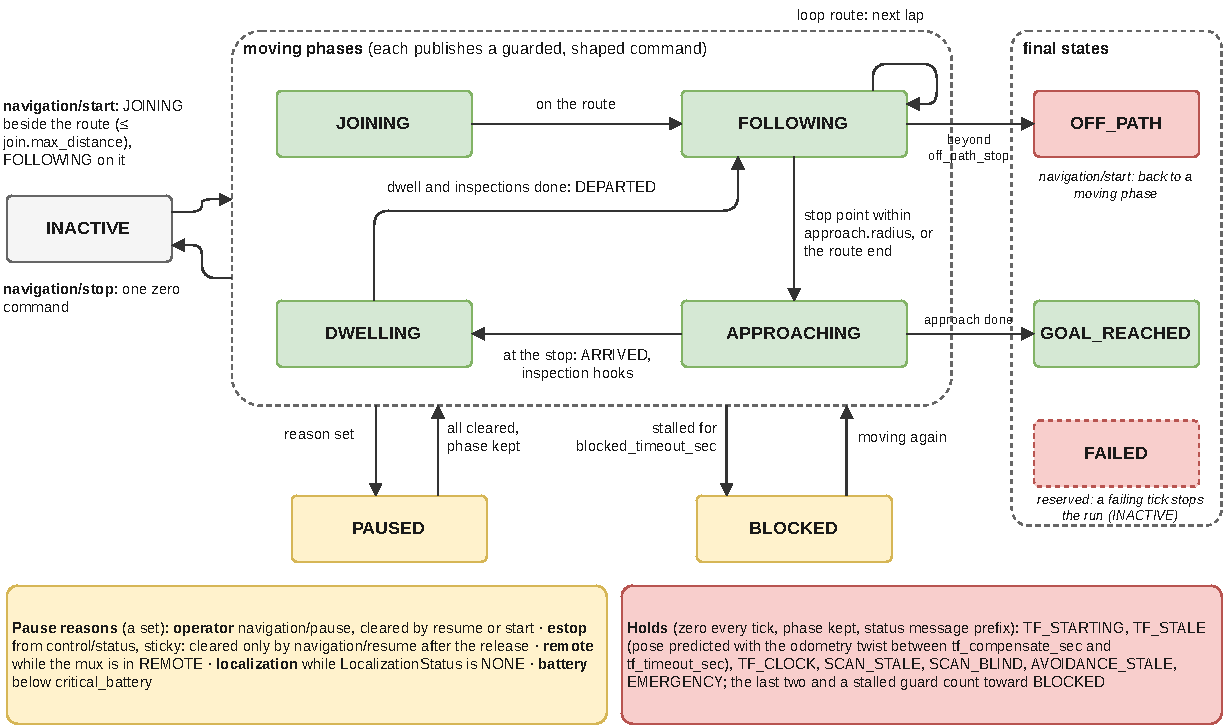
\includegraphics[width=\textwidth]{follower_fsm}
  \caption{States of the path follower, pause reasons and holds.}
  \label{fig:fsm}
\end{figure}

The follower is a pure state machine, \texttt{Follower.tick(inputs) -> Decision}: the node feeds it
the pose, the scans and the avoidance once per control tick and publishes the decision (command,
status, stop events). The states are the \code{NavigationStatus} constants and an explicit table
lists the allowed transitions (Fig.~\ref{fig:fsm}); a transition outside the table is a bug that
raises in the tests.

\subsection{Route, start and progress}

\topic{navigation/set_path} (planner) or the latched \topic{navigation/waypoints} (loader) give a
route of at least two points (review F17); a running follower starts over on a new route from
where the robot is. \topic{navigation/start} keeps the progress when the robot is still near it,
otherwise it locates the robot on the route, weighing the heading so the leg it walks along wins
over a parallel one. Beside the route (up to \param{join.max_distance}) it joins first
(\code{JOINING}); further away the start is refused. Start hooks (\param{hooks.start}) are called
asynchronously and the robot moves only when all succeeded.

Progress is searched in a short window ahead of the current one, against the line the robot is
meant to be on (route plus path offset), and its advance per tick is capped: a parallel leg never
captures it while the robot is shifted (review F5).

\subsection{Speed profile}

At each route point $i$ with curvature $\kappa_i$:
\begin{enumerate}
  \item curvature limit $v_i \le \sqrt{a_{\mathrm{lat}}/|\kappa_i|}$, clipped to
    $[v_{\min}, v_{\mathrm{cruise}}]$;
  \item approach speed at stop points and at the end;
  \item backward pass $v_i \le \sqrt{v_{i+1}^2 + 2 a_{\mathrm{dec}}\,\Delta s_i}$;
  \item the braking model \eqref{eq:m-braking}, reaction time included, before every stop;
  \item forward pass $v_{i+1} \le \sqrt{v_i^2 + 2 a_{\mathrm{acc}}\,\Delta s_i}$ out of the start
    and every stop (new in 0.2.0: the profile is consistent and predicts remaining time).
\end{enumerate}
Speeds and accelerations are capped by \param{robot.limits}. The speed regulator integrates a
signed error and resets on new paths; in 0.1 it integrated $|\omega| \ge 0$, so a positive gain
would have driven the speed to its minimum on long routes (finding N2).

\subsection{Controllers}

Controllers implement \code{PathController} and register in the \code{dharma.controllers}
registry; their parameters appear as \code{<name>.*} on the follower. Every controller applies
the avoidance the same way (finding N4): \code{heading_offset} (rad) rotates the commanded
direction of travel, \code{yaw_rate_bias} (rad/s) adds to the yaw rate.

\begin{center}
\begin{tabularx}{\textwidth}{@{}lX@{}}
  \toprule
  Controller & Law \\
  \midrule
  \code{holonomic} (default) & translation toward a carrot at arc length $s + L$ with
    $v = \min(v^*, \|\vect{c} - \vect{p}\|)$; heading toward the route direction a
    \code{heading_lookahead} ahead with a proportional, saturated yaw rate. The cross-track
    error obeys $\dot e = -v\,e/\sqrt{L^2 + e^2} \approx -(v/L)\,e$, so
    $e(t) = e_0 e^{-t/\tau}$ with $\tau = L/v$: 95\,\% after $3L$ of travel, independent of the
    speed. Lateral and heading loops are decoupled, which is why it does not oscillate on legged
    robots. \\
  \code{pure_pursuit}~\cite{coulter1992purepursuit} & curvature $2y/d^2$ toward the carrot at
    the requested speed \\
  \code{pid} & PID on the heading error toward the carrot, with a clamped integral
    (anti-windup, finding N2) \\
  \code{lqr} & error model $\vect{x} = [e_y, e_\psi]^\top$,
    $\vect{x}_{k+1} = \left[\begin{smallmatrix}1 & v\Delta t\\ 0 & 1\end{smallmatrix}\right]\vect{x}_k +
    \left[\begin{smallmatrix}0\\ \Delta t\end{smallmatrix}\right]u_k$, gain from the discrete Riccati
    equation per speed, $\omega = v\kappa - K\vect{x}$ \\
  \code{stanley}~\cite{thrun2006stanley} & $\omega = v\kappa - k_h\big(e_\psi +
    \arctan\frac{k\,e}{v + k_s}\big)$ toward the offset route \\
  \code{mppi}~\cite{williams2017mppi} & sampled yaw-rate sequences around the previous plan
    (warm start), unicycle rollouts, cost from route distance, carrot distance, intrusion into
    the clearance around the safety-scan points and effort, average $\vect{u}^* = \sum_i w_i
    \vect{u}_i$ with $w_i \propto \exp(-(J_i - J_{\min})/\lambda)$; seeded RNG (finding N2) \\
  \bottomrule
\end{tabularx}
\end{center}

\subsection{Path shift}

With \param{avoidance_mode} \code{path_shift} (omnidirectional robots), obstacle points of the
360° safety scan are expressed in route (Frenet) coordinates $(s, d)$~\cite{werling2010frenet}:
arc length along the route and signed distance to its left. A lateral offset $o$ is clear when no
point lies in the corridor
\begin{equation}
  |d - o| < w + c, \qquad s_{\mathrm{robot}} - b \le s \le s_{\mathrm{robot}} + f + \ell,
\end{equation}
($w$ half width, $c$ clearance, $b$, $f$ rear and front of the footprint, $\ell$ look-ahead).
Points beside the body block an offset outright; points ahead limit how far the robot can drive.
Among the candidates $o \in \{-o_{\max}, \ldots, o_{\max}\}$,
\begin{equation}
  o^* = \arg\min_{o\ \text{clear}}\ |o| + \lambda\,|o - o_{\mathrm{prev}}|,
\end{equation}
with a switch margin for other offsets than the current one; a move back toward the route is
taken only after it stayed proposed for \param{path_shift.return_delay_sec}. Without a clear
offset the robot keeps the one with the largest free distance (nearest the current one on ties)
and slows. The commanded offset moves toward the target at \param{path_shift.offset_rate}. The
speed limit is $v^*(d_{\mathrm{free}} - m)$ where $d_{\mathrm{free}}$ is the smallest free
distance over the target offset, the commanded offset \emph{and the measured lateral offset}
(review F4), so a robot still sliding is not sped up by the offset it has not reached. A blind
scan stops the robot. Near a stop point it stays on the route and waits for an obstacle instead
of passing it (review F6).

\subsection{Reactive avoidance}

With \code{reactive}, \code{obstacle_avoidance_node} runs one policy of the
\code{dharma.avoidance} registry on \topic{perception/sector_scan} and publishes an
\code{AvoidanceCommand}: heading offset (rad), yaw-rate bias (rad/s), lateral bias (m/s, omni),
speed scale and an emergency flag (an obstacle closer than \param{shared.emergency_distance} in
the cone $\pm$\param{shared.emergency_cone_deg}). Blocked sectors are obstacles.
\begin{center}
\begin{tabularx}{\textwidth}{@{}lX@{}}
  \toprule
  Policy & Principle \\
  \midrule
  \code{braitenberg} & danger left and right steers, danger ahead or beside slows \\
  \code{vfh}~\cite{borenstein1991vfh} (default) & only when the frontal cone is blocked, aim at
    the nearest edge of a wide enough gap \\
  \code{potential_field}~\cite{khatib1986potential} & obstacles inside the safe distance repel,
    $\vect{F} = -\sum_j \eta\big(\tfrac{1}{r_j} - \tfrac{1}{r_0}\big)\tfrac{1}{r_j^2}\hat{\vect{u}}_j$;
    the sideways part steers and pushes, danger ahead slows \\
  \code{follow_gap}~\cite{sezer2012ftg} & bubble the nearest obstacle, aim at the centre of the
    widest gap \\
  \bottomrule
\end{tabularx}
\end{center}
The outputs are smoothed asymmetrically: the speed scale drops at once and only rises through
the filter, the emergency flag is never filtered (review F13).

\textbf{Is the emergency cone enough?} With $\tr = 0.25$~s the stopping distances are
\begin{center}
\begin{tabular}{@{}lrrl@{}}
  \toprule
  $v$ & $a = 0.5$ & $a = 0.6$ & 0.35~m of room? \\
  \midrule
  0.35~m/s (cruise in 0.1) & 0.21~m & 0.19~m & yes \\
  0.60~m/s & 0.51~m & 0.45~m & no \\
  1.0~m/s & 1.25~m & 1.08~m & no \\
  \bottomrule
\end{tabular}
\end{center}
so the cone (0.75~m from \frm{base_link}, about 0.35~m from the nose) is a second line; the motion
guard and the protective field limit the speed before.

\subsection{Stop points}

Stop points (\texttt{dwell\_sec > 0}) are detected by progress (within \param{approach.radius} along
the route) and by distance minus the path offset; a stop on a later leg that passes close never
triggers early, and one is skipped only once the progress passed it by
\param{approach.skip_margin} (review F6). At a stop: final x, y, yaw approach, \code{ARRIVED},
inspection hooks (asynchronous; answers for an earlier stop or route are dropped), dwell,
\code{DEPARTED}. Route processing keeps stop points closer than 3~cm apart (review F12).

\subsection{Supervisor, motion guard and command shaper}

\begin{itemize}
  \item \textbf{Pose.} \code{TF_STARTING} without a pose; \code{TF_STALE} above
    \param{safety.tf_timeout_sec}; between \param{safety.tf_compensate_sec} and the timeout the
    pose is predicted forward with the odometry twist instead of stopping; \code{TF_CLOCK} for a
    pose from the future (clock mismatch).
  \item \textbf{Scans and avoidance.} \code{SCAN_STALE}, \code{SCAN_BLIND} (blocked sectors),
    \code{AVOIDANCE_STALE}, \code{EMERGENCY} (held for \param{safety.emergency_release_sec}).
  \item \textbf{Blocked and off path.} No progress for \param{safety.blocked_timeout_sec} is
    \code{BLOCKED}; more than \param{safety.off_path_stop} from the route beyond the path offset is
    \code{OFF_PATH} (the robot slows from \param{safety.off_path_slow}).
  \item \textbf{Motion guard.} Every command, in every phase (following, joining, final
    approach), is limited along its direction by the 360° safety scan with the footprint and the
    braking model, and the yaw rate by the free turning angle (review F7; 0.1 checked joining
    and the final approach with the front cone only).
  \item \textbf{Command shaper.} Robot envelope (x and y scaled together, $v_y = 0$ for diff
    robots), smoothing of yaw rate and sideways speed, slew limits from \param{robot.limits},
    non-finite values to zero (review F11).
\end{itemize}
Zero commands are published once on entering \code{INACTIVE} or a final state, every tick while
paused or held, on stop, on shutdown (a hook) and when a control tick raises (review F2). All
state-changing callbacks and the control loop share one mutually exclusive callback group and a
lock (review F3); timers (dwell, approach) are frozen while paused (review F7).

\subsection{Pause reasons}

A set of reasons, each with its own way of clearing (review F16):
\begin{center}
\begin{tabularx}{\textwidth}{@{}lX@{}}
  \toprule
  Reason & Set and cleared \\
  \midrule
  \code{operator} & \topic{navigation/pause}; cleared by \topic{navigation/resume} or start \\
  \code{estop} & \topic{control/status} reports the e-stop; sticky: cleared only by
    \topic{navigation/resume} after the release, so the robot never drives off on its own after
    an e-stop \\
  \code{remote} & while the mux is in REMOTE \\
  \code{localization} & while \topic{localization/status} is \code{NONE}; cleared when localized
    again \\
  \code{battery} & below \param{critical_battery}; below \param{low_battery} a loop route finishes
    its lap and stops \\
  \bottomrule
\end{tabularx}
\end{center}
Start is refused while \code{estop} or \code{localization} hold.

\section{Interfaces}

\begin{center}
\begin{tabularx}{\textwidth}{@{}p{0.36\textwidth}p{0.24\textwidth}X@{}}
  \toprule
  Interface & Type & \\
  \midrule
  \topic{planner/go_to}, \topic{planner/plan} & GoTo, PlanPath & plan (and drive) to x, y, yaw \\
  \topic{planner/cancel} & Trigger & \\
  \topic{planner/status}, \topic{planner/path}, \topic{planner/costmap} & PlannerStatus, Path,
    OccupancyGrid & latched \\
  \topic{navigation/set_path}, \topic{navigation/load_path} & SetPath, LoadPath & \\
  \topic{navigation/start}, \topic{stop}, \topic{pause}, \topic{resume} & Trigger & \\
  \topic{navigation/status} & NavigationStatus, latched & state, pause reasons, progress \\
  \topic{navigation/stop_point} & StopPointEvent & \\
  \topic{navigation/waypoints}, \topic{navigation/path} & WaypointPath, Path & loaded route \\
  \topic{navigation/avoidance} & AvoidanceCommand & avoidance $\to$ follower \\
  \topic{control/nav_cmd_vel} & Twist & to the control mux \\
  in: \topic{/map}, \topic{perception/safety_scan}, \topic{perception/sector_scan},
    \topic{control/status}, \topic{localization/status}, battery, odom & & \\
  \bottomrule
\end{tabularx}
\end{center}

\section{Parameters}

\readonlynote

% Generated by docs/manual/tools/reference.py; do not edit.
\begin{small}
\begin{longtable}{@{}>{\raggedright}p{0.25\textwidth}>{\raggedright}p{0.17\textwidth}>{\raggedright}p{0.10\textwidth}>{\raggedright}p{0.11\textwidth}>{\raggedright\arraybackslash}p{0.25\textwidth}@{}}
\toprule
Parameter & Default & Unit & Range & Description \\
\midrule
\endhead
\bottomrule
\endfoot
\multicolumn{5}{@{}l}{\textbf{planner\_\allowbreak{}node}} \\
\code{costmap.resolution} & 0.1 & m & 0.01..1 & planning cell size, the map is max-pooled to it \\
\code{costmap.margin} & 0.1 & m & 0..1 & clearance added to the footprint (keep >= half a cell) \\
\code{costmap.inflation_radius} & 0.8 & m & 0..5 & paths keep away from walls up to here \\
\code{costmap.cost_scaling} & 3 & 1/\allowbreak{}m & 0..50 & how fast the wall cost falls off \\
\code{costmap.unknown_is_obstacle} & true &  &  & never plan through unmapped space \\
\code{costmap.occupied_threshold} & 50 &  & 1..100 & map values from here are obstacles \\
\code{search.goal_tolerance} & 0.5 & m & 0..5 & a goal in an obstacle moves to free space this close \\
\code{search.start_escape} & 1 & m & 0..5 & a robot inside the inflation walks out up to here \\
\code{search.heuristic_weight} & 1 &  & 1..5 & > 1: faster search, slightly longer paths \\
\code{search.timeout_sec} & 5 & s & 0.1..60 & search time limit \\
\code{search.spacing} & 0.1 & m & 0.02..1 & distance between waypoints \\
\code{search.smooth_weight_data} & 0.1 &  & 0..1 & pull toward the search path \\
\code{search.smooth_weight_smooth} & 0.3 &  & 0..0.49 & pull toward the neighbours \\
\code{search.footprint_retries} & 5 &  & 0..20 & searches around poses where the oriented footprint collides \\
\code{monitor.arrival_tolerance} & 0.35 & m & 0.01..5 & GOAL\_\allowbreak{}REACHED counts this close to the plan goal \\
\code{monitor.stop_on_arrival} & true &  &  & stop the follower at the goal \\
\code{monitor.replan_after_sec} & 3 & s & 0.1..300 & follower BLOCKED this long: plan again \\
\code{monitor.max_replans} & 5 &  & 0..100 & per goal, then failed \\
\code{monitor.cancel_after_sec} & 1 & s & 0.1..60 & follower INACTIVE this long: cancelled \\
\code{use_live_obstacles} & true &  &  & replans see the obstacles of the safety scan \\
\code{scan_timeout_sec}$^\dagger$ & 1 & s & 0.05..10 & older safety scans are ignored \\
\code{tf_timeout_sec}$^\dagger$ & 0.5 & s & 0.05..10 & an older robot pose is unknown \\
\code{publish_costmap} & false &  &  & planner/costmap for RViz (debug) \\
\code{status_hz} & 2 & Hz & 0.1..50 & planner/status while active \\
\code{service_timeout_sec} & 5 & s & 0.1..60 & calls to the follower \\
\multicolumn{5}{@{}l}{\textbf{path\_\allowbreak{}loader\_\allowbreak{}node}} \\
\code{sites_dir}$^\dagger$ & \code{~/dharma/map} &  &  & routes are loaded from inside this directory only \\
\code{route}$^\dagger$ & \code{""} &  &  & route CSV loaded at start (inside sites\_\allowbreak{}dir) \\
\code{remember_file}$^\dagger$ & \code{~/.dharma/last_route} &  &  & last loaded route, reloaded at start ("": off) \\
\code{process} & true &  &  & resample and smooth routes between stop points \\
\code{processing.spacing} & 0.1 & m & 0.02..1 & point spacing after resampling \\
\code{processing.smooth_weight_data} & 0.05 &  & 0..1 & pull toward the recording \\
\code{processing.smooth_weight_smooth} & 0.4 &  & 0..0.49 & pull toward neighbours \\
\code{processing.max_deviation} & 0.3 & m & 0..5 & warn when smoothing moves the route further \\
\code{republish_sec} & 2 & s & 0..60 & navigation/path republish for RViz (0: off) \\
\multicolumn{5}{@{}l}{\textbf{path\_\allowbreak{}follower\_\allowbreak{}node}} \\
\code{control_rate}$^\dagger$ & 20 & Hz & 1..200 & loop rate \\
\code{controller} & \code{holonomic} &  &  & path controller (dharma.controllers) \\
\code{avoidance_mode} & \code{path_shift} &  & path\_\allowbreak{}shift, reactive, off & path\_\allowbreak{}shift: slide sideways (holonomic) \\
\code{loop_route} & false &  &  & restart a closed route at its end (patrol) \\
\code{loop_close_distance} & 1 & m & 0..20 & end this close to the start: a closed route \\
\code{require_localization} & true &  &  & pause while localization/status is NONE \\
\code{low_battery} & 0.2 &  & 0..1 & below: finish the lap, no new one \\
\code{critical_battery} & 0.1 &  & 0..1 & below: pause (reason battery) \\
\code{battery_hysteresis} & 0.05 &  & 0..0.5 & recharge above + this \\
\code{speed.cruise} & 0.4 & m/\allowbreak{}s & 0.01..5 & cruise speed \\
\code{speed.min_speed} & 0.1 & m/\allowbreak{}s & 0..5 & floor of the curve limit \\
\code{speed.approach_speed} & 0.15 & m/\allowbreak{}s & 0.01..5 & speed at stop points and the route end \\
\code{speed.lateral_accel} & 0.3 & m/\allowbreak{}s$^{2}$ & 0.01..10 & curve limit v = sqrt(a / curvature) \\
\code{speed.accel} & 0.3 & m/\allowbreak{}s$^{2}$ & 0.01..20 & comfortable acceleration \\
\code{speed.decel} & 0.3 & m/\allowbreak{}s$^{2}$ & 0.01..20 & comfortable braking \\
\code{speed.smoothing} & 0.5 &  & 0.05..1 & weight of a new yaw rate / sideways command (1: off) \\
\code{safety.stop_margin}$^\dagger$ & 0.3 & m & 0..5 & gap kept to obstacles when stopping \\
\code{safety.yaw_margin_deg}$^\dagger$ & 5 & deg & 0..90 & turning room kept to obstacles \\
\code{safety.scan_timeout_sec}$^\dagger$ & 0.5 & s & 0.05..5 & older safety scans stop the robot \\
\code{safety.avoidance_timeout_sec}$^\dagger$ & 0.5 & s & 0.05..5 & older avoidance (reactive) stops it \\
\code{safety.tf_timeout_sec}$^\dagger$ & 0.5 & s & 0.05..5 & an older pose stops the robot \\
\code{safety.tf_compensate_sec}$^\dagger$ & 0.1 & s & 0..5 & older poses are predicted forward \\
\code{safety.clock_tolerance_sec}$^\dagger$ & 0.1 & s & 0..5 & a pose from further in the future: clock \\
\code{safety.emergency_release_sec} & 1 & s & 0..30 & an emergency stop holds this long after it clears \\
\code{safety.blocked_timeout_sec} & 10 & s & 0.5..600 & no progress this long: BLOCKED \\
\code{safety.off_path_slow} & 0.6 & m & 0.05..10 & further from the route: slow to the floor speed \\
\code{safety.off_path_stop} & 1.5 & m & 0.1..20 & further from the route: OFF\_\allowbreak{}PATH, stopped \\
\code{path_shift.max_offset} & 0.8 & m & 0..5 & furthest from the route \\
\code{path_shift.step} & 0.1 & m & 0.02..1 & candidate offset spacing \\
\code{path_shift.look_ahead} & 2 & m & 0.1..20 & route ahead of the front edge that must be free \\
\code{path_shift.clearance} & 0.1 & m & 0..2 & gap kept beside the body \\
\code{path_shift.offset_rate} & 0.3 & m/\allowbreak{}s & 0.01..5 & how fast it slides onto a new offset \\
\code{path_shift.switch_cost} & 0.5 &  & 0..10 & keeps its side (hysteresis) \\
\code{path_shift.switch_margin} & 0.05 & m & 0..1 & extra clearance a new offset needs \\
\code{path_shift.return_delay_sec} & 0.5 & s & 0..30 & a way back must stay proposed this long \\
\code{path_shift.stop_margin} & 0.4 & m & 0..5 & stop this far before an obstacle (front edge) \\
\code{approach.radius} & 0.5 & m & 0.05..5 & this close (along the route) the approach starts \\
\code{approach.skip_margin} & 0.5 & m & 0.05..10 & progress this far past a stop: skipped \\
\code{approach.timeout_sec} & 20 & s & 1..600 & give up converging (paused time not counted) \\
\code{approach.kp_xy} & 1.2 & 1/\allowbreak{}s & 0..10 & gain on the position error \\
\code{approach.kp_yaw} & 1.5 & 1/\allowbreak{}s & 0..10 & gain on the yaw error \\
\code{approach.max_speed} & 0.2 & m/\allowbreak{}s & 0.01..2 & approach speed cap \\
\code{approach.max_yaw_rate} & 0.6 & rad/\allowbreak{}s & 0.01..5 & yaw rate cap \\
\code{approach.min_speed} & 0.04 & m/\allowbreak{}s & 0..1 & floor to beat the robot deadband \\
\code{approach.position_tolerance} & 0.05 & m & 0.005..1 & arrived within \\
\code{approach.yaw_tolerance_deg} & 3 & deg & 0.1..45 & aligned within \\
\code{join.max_distance} & 3 & m & 0..50 & a robot this far walks onto the route (0: off) \\
\code{join.timeout_sec} & 60 & s & 1..600 & give up and follow from where it is \\
\code{join.on_route} & 0.15 & m & 0.01..2 & joined within this \\
\code{hooks.start}$^\dagger$ & [] &  &  & called on start; the robot waits for every success \\
\code{hooks.stop}$^\dagger$ & [] &  &  & called on stop (not waited for) \\
\code{hooks.inspection}$^\dagger$ & [] &  &  & called at every stop point \\
\code{hooks.timeout_sec}$^\dagger$ & 5 & s & 0.1..120 & start and stop hook timeout \\
\code{hooks.inspection_timeout_sec} & 20 & s & 0.1..600 & a stop waits this long for inspections \\
\code{regulator.enabled} & false &  &  & scale the speed down when turning hard \\
\code{regulator.reference_yaw_rate} & 0.3 & rad/\allowbreak{}s & 0..5 & turning slower than this needs no slow-down \\
\code{regulator.kp} & 0.5 & s/\allowbreak{}rad & 0..10 & scale per rad/s above it \\
\code{regulator.ki} & 0 & 1/\allowbreak{}rad & 0..10 & scale per integrated rad \\
\code{regulator.integral_limit} & 1 & rad & 0..10 & anti-windup clamp \\
\code{regulator.min_scale} & 0.3 &  & 0..1 & never slower than this fraction \\
\code{processing.spacing} & 0.1 & m & 0.02..1 & point spacing after resampling \\
\code{processing.smooth_weight_data} & 0.05 &  & 0..1 & pull toward the recording \\
\code{processing.smooth_weight_smooth} & 0.4 &  & 0..0.49 & pull toward neighbours \\
\code{processing.max_deviation} & 0.3 & m & 0..5 & warn when smoothing moves the route further \\
\code{markers} & true &  &  & publish RViz markers \\
\multicolumn{5}{@{}l}{\textbf{obstacle\_\allowbreak{}avoidance\_\allowbreak{}node}} \\
\code{policy} & \code{vfh} &  &  & avoidance policy (dharma.avoidance) \\
\code{shared.safe_distance} & 1 & m & 0.1..20 & obstacles closer than this shape the command \\
\code{shared.emergency_distance} & 0.75 & m & 0..10 & obstacle in the cone closer than this: stop \\
\code{shared.emergency_cone_deg} & 60 & deg & 1..360 & frontal cone of the emergency stop \\
\code{shared.max_heading_offset_deg} & 60 & deg & 0..180 & largest turn of the direction of travel \\
\code{shared.smoothing} & 0.8 &  & 0..0.99 & 0..1 filter on steering and speeding up (never on braking) \\
\code{braitenberg.steering_gain} & 1 & rad & 0..10 & turn per unit danger \\
\code{braitenberg.velocity_gain} & 1 &  & 0..10 & slow-down per unit danger \\
\code{braitenberg.steering_zone_center_deg} & 45 & deg & 0..180 &  \\
\code{braitenberg.steering_zone_width_deg} & 60 & deg & 1..360 &  \\
\code{braitenberg.velocity_zone_center_deg} & 60 & deg & 0..180 &  \\
\code{braitenberg.velocity_zone_width_deg} & 90 & deg & 1..360 &  \\
\code{braitenberg.following_zone_width_deg} & 30 & deg & 1..360 &  \\
\code{vfh.min_gap_width_deg} & 20 & deg & 1..180 & narrowest passable gap \\
\code{vfh.steering_gain} & 1 &  & 0..5 & fraction of the gap heading taken \\
\code{vfh.velocity_gain} & 1 &  & 0..10 & slow-down per unit frontal danger \\
\code{potential_field.repulsion_gain} & 0.5 &  & 0..10 & strength of the repulsion \\
\code{potential_field.steering_gain} & 0.8 & rad & 0..5 & turn per atan(force) \\
\code{potential_field.lateral_gain} & 0.3 &  & 0..5 & sideways m/s per unit force \\
\code{potential_field.max_lateral} & 0.2 & m/\allowbreak{}s & 0..2 & cap on the sideways push \\
\code{potential_field.velocity_gain} & 1 &  & 0..10 & slow-down per unit frontal danger \\
\code{follow_gap.bubble_radius} & 0.45 & m & 0..5 & safety bubble around the nearest obstacle \\
\code{follow_gap.steering_gain} & 1 &  & 0..5 & fraction of the gap heading taken \\
\code{follow_gap.velocity_gain} & 1 &  & 0..10 & slow-down per unit frontal danger \\
\code{markers} & true &  &  & publish RViz markers \\
\end{longtable}
\end{small}


\subsection{Controller parameters}

% Generated by docs/manual/tools/reference.py; do not edit.
\begin{small}
\begin{longtable}{@{}p{0.28\textwidth}p{0.12\textwidth}p{0.08\textwidth}p{0.11\textwidth}p{0.29\textwidth}@{}}
\toprule
Parameter & Default & Unit & Range & Description \\
\midrule
\endhead
\bottomrule
\endfoot
\multicolumn{5}{@{}l}{\textbf{path\_follower\_node: holonomic}} \\
\code{holonomic.lookahead} & 0.6 & m & 0.1\,..\,5 & carrot ahead along the route; longer = gentler \\
\code{holonomic.heading_lookahead} & 0.6 & m & 0.1\,..\,5 & the heading follows the route this far ahead \\
\code{holonomic.kp_yaw} & 1.5 & 1/s & 0\,..\,10 & yaw rate per rad of error \\
\code{holonomic.max_lateral_speed} & 0.25 & m/s & 0\,..\,5 & sideways speed cap (0: never strafe) \\
\code{holonomic.max_reverse_speed} & 0.15 & m/s & 0\,..\,5 & backward speed cap when the route is behind \\
\code{holonomic.min_alignment_scale} & 0.25 &  & 0\,..\,1 & translation factor while the heading is far off \\
\multicolumn{5}{@{}l}{\textbf{path\_follower\_node: pure\_pursuit}} \\
\code{pure_pursuit.lookahead} & 1 & m & 0.1\,..\,5 & carrot ahead along the route \\
\multicolumn{5}{@{}l}{\textbf{path\_follower\_node: pid}} \\
\code{pid.lookahead} & 1 & m & 0.1\,..\,5 & carrot ahead along the route \\
\code{pid.kp} & 1.5 & 1/s & 0\,..\,20 & proportional gain \\
\code{pid.ki} & 0 & 1/s$^{2}$ & 0\,..\,20 & integral gain \\
\code{pid.kd} & 0.2 &  & 0\,..\,20 & derivative gain \\
\code{pid.integral_limit} & 0.5 & rad s & 0\,..\,10 & anti-windup clamp of the error integral \\
\multicolumn{5}{@{}l}{\textbf{path\_follower\_node: lqr}} \\
\code{lqr.q_lateral} & 1 &  & 0\,..\,100 & weight on the cross-track error \\
\code{lqr.q_heading} & 0.5 &  & 0\,..\,100 & weight on the heading error \\
\code{lqr.r_yaw_rate} & 0.5 &  & 0.001\,..\,100 & weight on the yaw rate (higher = gentler) \\
\multicolumn{5}{@{}l}{\textbf{path\_follower\_node: stanley}} \\
\code{stanley.k_cross_track} & 1 &  & 0\,..\,20 & cross-track gain \\
\code{stanley.k_soft} & 0.2 & m/s & 0.01\,..\,5 & softening so low speeds do not over-steer \\
\code{stanley.k_heading} & 1.5 & 1/s & 0\,..\,20 & steering to yaw rate gain \\
\multicolumn{5}{@{}l}{\textbf{path\_follower\_node: mppi}} \\
\code{mppi.horizon_steps} & 15 &  & 2\,..\,100 & steps per rollout \\
\code{mppi.step_sec} & 0.1 & s & 0.01\,..\,1 & rollout step \\
\code{mppi.samples} & 200 &  & 10\,..\,5000 & rollouts per tick \\
\code{mppi.yaw_rate_std} & 1 & rad/s & 0.01\,..\,5 & sampling noise \\
\code{mppi.temperature} & 0.05 &  & 0.001\,..\,100 & softmax sharpness of the normalized cost \\
\code{mppi.window} & 4 & m & 0.5\,..\,20 & route ahead in the cost \\
\code{mppi.obstacle_weight} & 5 &  & 0\,..\,1000 & cost per m of intrusion \\
\code{mppi.clearance} & 0.5 & m & 0\,..\,5 & rollouts closer to an obstacle pay for it \\
\code{mppi.seed}$^\dagger$ & 0 &  & 0\,..\,2.14748e+09 & random seed (reproducible) \\
\end{longtable}
\end{small}

